\documentclass{article}
\usepackage{preamble}

\title{ENGR3426: Miniproject 1}
\author{Jacob Smilg}
\date{September 12th 2023}

\urlstyle{same}
\begin{document}

\maketitle

\section{Schematic Capture and Simulation}

\begin{figure}[!ht]
    \centering
    \includesvg[inkscapelatex=false, width=.9\columnwidth]{../images/AND2_tran.svg}
    \caption{Schematic of my 2-input AND gate simulation test harness created in Xschem. The parameters used for \texttt{pulse()} for sources Va and Vb were chosen such that they will cycle through all possible input combinations.}\label{fig:and_sim_schem}
\end{figure}

\captionsetup[subfigure]{margin=10pt}

\begin{figure}[!ht]
    \centering
    \begin{subfigure}{.5\textwidth}
        \centering
        \includesvg[inkscapelatex=false, width=.6\linewidth]{../images/inverter.svg}
        \caption{Schematic of my CMOS inverter created in Xschem.}\label{fig:inverter_schem}
    \end{subfigure}%
    \begin{subfigure}{.5\textwidth}
        \centering
        \includesvg[inkscapelatex=false, width=.7\linewidth]{../images/NAND2.svg}
        \caption{Schematic of my 2-input NAND gate created in Xschem.}\label{fig:nand_schem}
    \end{subfigure}
\end{figure}

\begin{figure}[p]
    \centering
    \includesvg[inkscapelatex=false, width=.8\columnwidth]{../images/simplot.svg}
    \caption{A plot of the output of the simulation of Figure~\ref{fig:and_sim_schem}. The AND gate behaves as expected; its output is only high when Va and Vb are high, and there is a small delay (approximately 1ns) between the input and output.}\label{fig:simplot}
\end{figure}
\pagebreak

\section{Layout Design}

\begin{figure}[h]
    \centering
    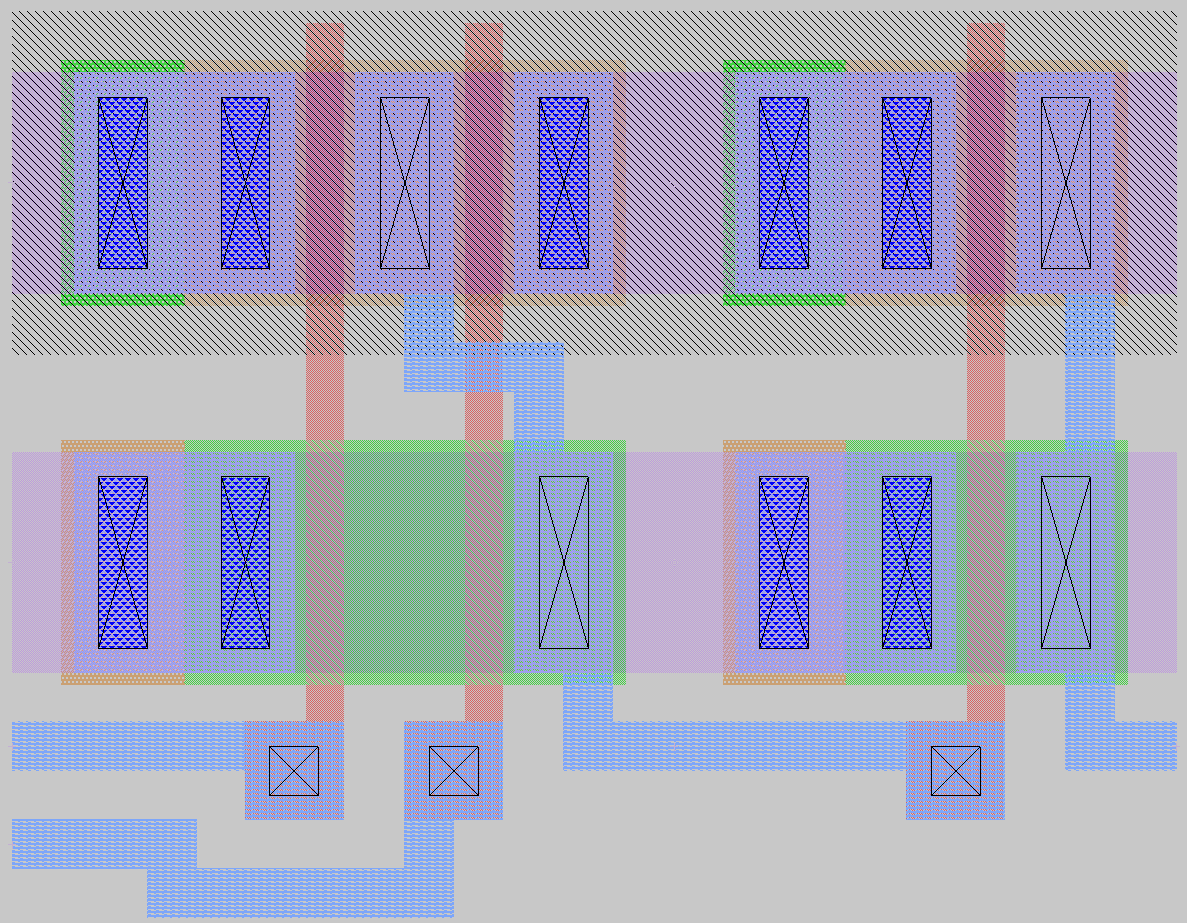
\includegraphics[width=\columnwidth]{../images/magic-layout.png}
    \caption{A screenshot of the top-level cell layout of my 2-input AND gate.}\label{fig:layout}
\end{figure}
\pagebreak

\section{Layout Versus Schematic}

\begin{figure}[h]
    \centering
    \includesvg[inkscapelatex=false, width=.9\columnwidth]{../images/AND2.svg}
    \caption{Schematic of my 2-input AND gate separated from the simulation test harness for LVS. Note that the bulk connections of the NAND gate MOSFETs were manually set to VP and VN in the symbol properties to prevent extraneous VDD and GND nets from being created.}\label{fig:and_lvs_schem}
\end{figure}
\pagebreak

\subsection{LVS Output Log}

The following is the contents of the file \texttt{mp1/layout/comp.out} obtained from running the netgen LVS program comparing \texttt{mp1/layout/AND2.spice} (Magic netlist) and \texttt{mp1/simulation/AND2.spice} (Xschem netlist). It shows that the layout and schematic match.

\lstset{%
    breaklines=true,
    breakatwhitespace=true,
}
\lstinputlisting{../layout/comp.out}

\section{Design Files}

All of the files for this miniproject can be found at \url{https://github.com/smilg/madvlsi-fa23/tree/main/mp1}.

\end{document}